\documentclass[12pt]{article}

\usepackage[a4paper, margin=1in]{geometry}
\usepackage{graphicx}
\usepackage{float}
\usepackage[hidelinks]{hyperref}

\setlength{\parindent}{0pt}
\setlength{\parskip}{5pt}
\setlength{\intextsep}{6pt}
\setlength{\textfloatsep}{6pt}
\setlength{\abovecaptionskip}{3pt}
\setlength{\belowcaptionskip}{3pt}

\title{\textbf{Mini Game Hub Report}}
\author{\textbf{Made by AMAN SIHAG AND AKSHIT}}
\date{\today}

\begin{document}

\maketitle
\thispagestyle{empty}
\clearpage

\tableofcontents
\thispagestyle{empty}
\clearpage

\section{Project Specification}

\textbf{Technologies Used:}
\begin{itemize}
    \item Bash
    \item Python 3.10
    \item Pygame
    \item NumPy
    \item Matplotlib
\end{itemize}

\section{Overview}

The Mini Game Hub is a secure multiplayer gaming platform where two authenticated users can play multiple games through a graphical interface. The system integrates Bash for authentication and Python for game execution, data recording, and analytics.

\section{System Architecture}

\begin{verbatim}
hub/
|-- main.sh
|-- game.py
|-- leaderboard.sh
|-- games/
|   |-- tictactoe.py
|   |-- othello.py
|   |-- connect4.py
|-- users.tsv
|-- history.csv
\end{verbatim}

\textbf{Entry point:}
\begin{verbatim}
bash main.sh
\end{verbatim}

\section{Authentication System}

\begin{itemize}
    \item Two users are authenticated using SHA-256 hashing.
    \item Passwords are securely stored (not plaintext).
    \item New users can register.
    \item After login, Python game engine is launched.
\end{itemize}

\begin{verbatim}
python3 game.py <username1> <username2>
\end{verbatim}

\section{Game Engine}

The system uses a base class for all games:
\begin{itemize}
    \item Player handling
    \item Turn switching
    \item NumPy-based board
    \item Win condition checking
\end{itemize}

\section{Games Implemented}

\subsection{Tic Tac Toe}
\begin{itemize}
    \item 10×10 grid
    \item Win condition: 5 in a row
\end{itemize}

\subsection{Othello}
\begin{itemize}
    \item 8×8 board
    \item Disc flipping mechanics
\end{itemize}

\subsection{Connect Four}
\begin{itemize}
    \item 7×7 grid
    \item Gravity-based coin placement
\end{itemize}

\section{Screenshots and UI}

\subsection{Game Menu}
\begin{figure}[H]
    \centering
    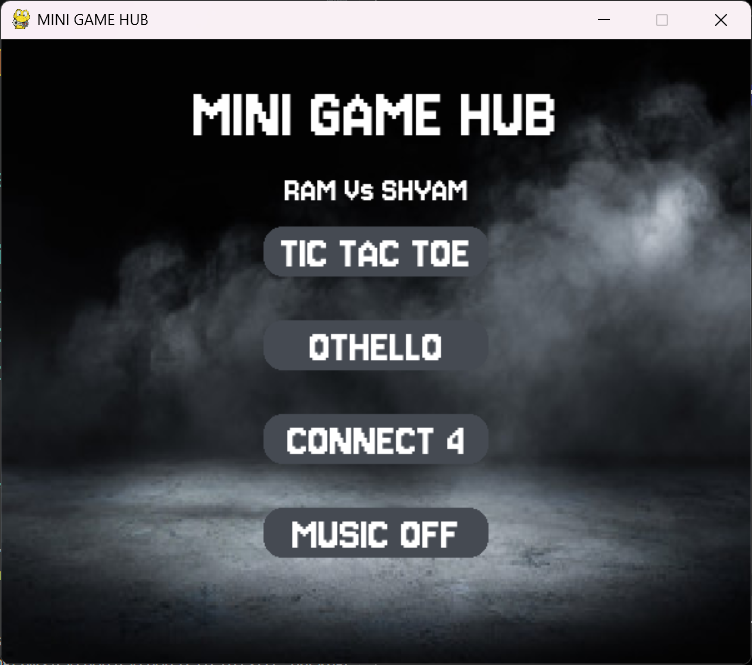
\includegraphics[width=0.75\linewidth]{images/menu.png}
    \caption{Main Game Menu}
\end{figure}

\subsection{Tic Tac Toe}
\begin{figure}[H]
    \centering
    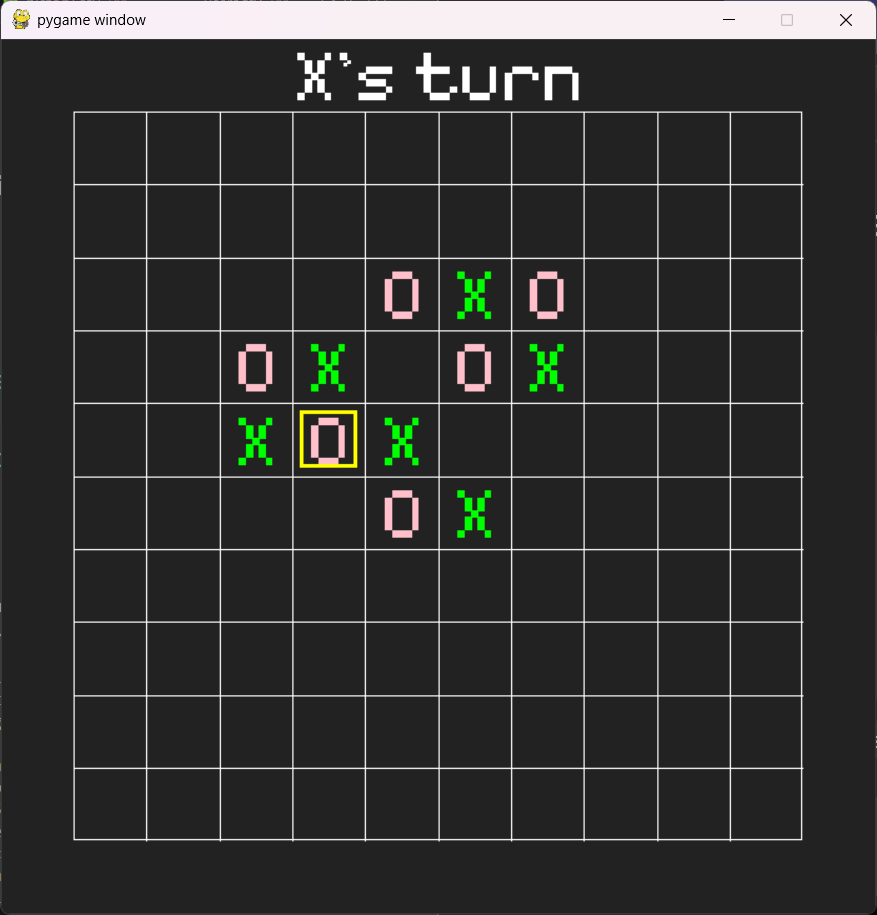
\includegraphics[width=0.75\linewidth]{images/tictactoe.png}
    \caption{Tic Tac Toe Gameplay}
\end{figure}

\subsection{Game Over}
\begin{figure}[H]
    \centering
    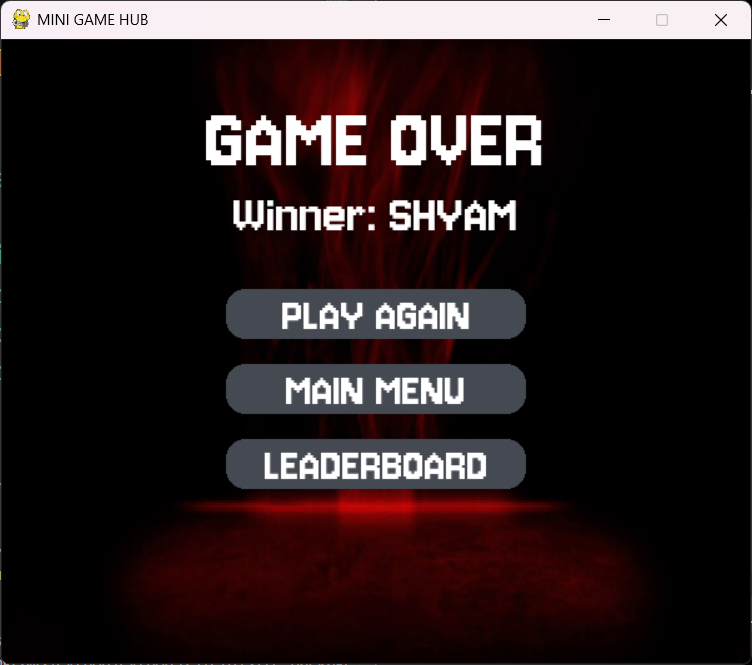
\includegraphics[width=0.75\linewidth]{images/gameover.png}
    \caption{Game Over Screen}
\end{figure}

\subsection{Leaderboard}
\begin{figure}[H]
    \centering
    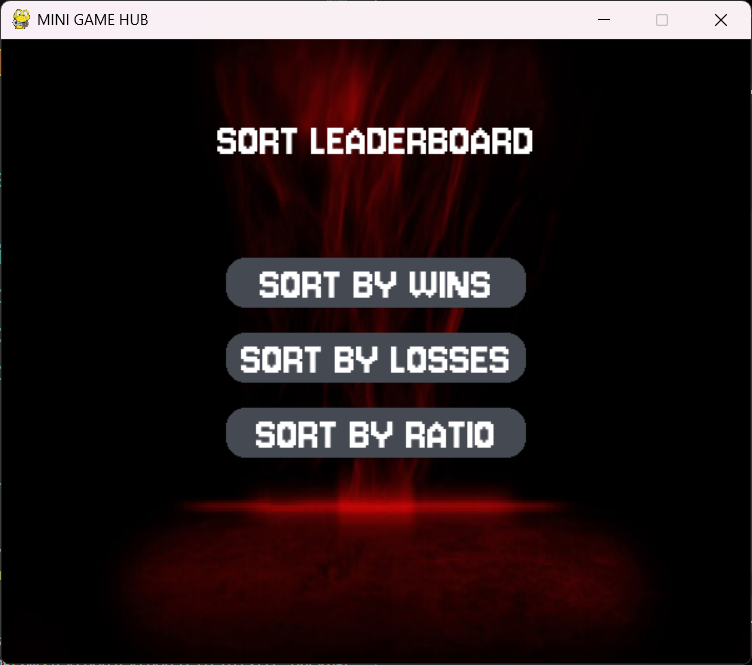
\includegraphics[width=0.75\linewidth]{images/leaderboard.png}
    \caption{Leaderboard Interface}
\end{figure}

\subsection{Graphs}
\begin{figure}[H]
    \centering
    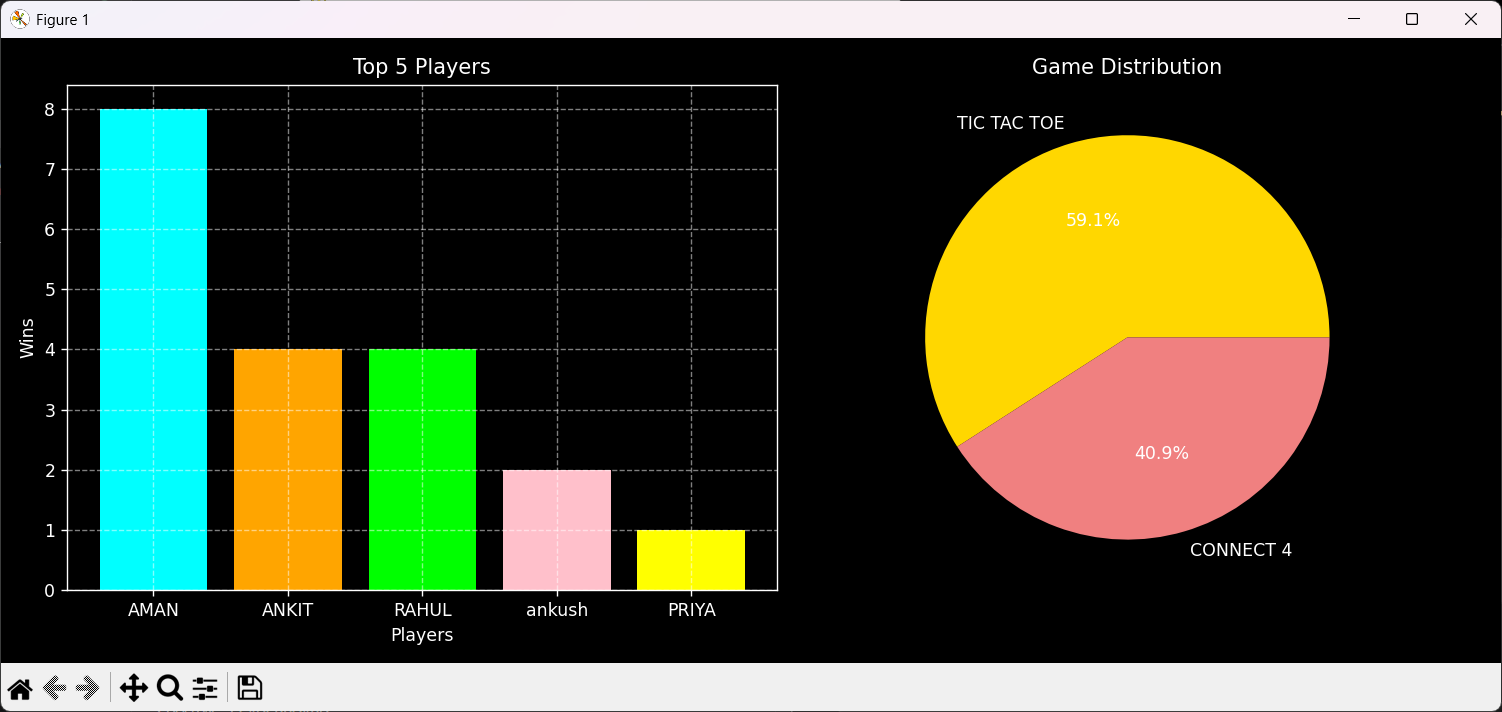
\includegraphics[width=0.75\linewidth]{images/graphs.png}
    \caption{Statistical Graphs}
\end{figure}

\section{Leaderboard and Analytics}

\begin{itemize}
    \item Game results are stored in history.csv
    \item Leaderboard is generated using Bash
    \item Displays wins, losses, and ratios
\end{itemize}

\section{Technical Constraints}

\begin{itemize}
    \item NumPy used for all board representations
    \item Win logic implemented using vectorized operations
    \item No manual loops for win checking
    \item Full GUI using Pygame
\end{itemize}

\section{Hurdles Faced}

\begin{itemize}
    \item Integrating Bash with Python
    \item Handling real-time UI in Pygame
    \item Implementing NumPy-based logic
    \item Managing CSV data consistency
\end{itemize}

\textbf{Solutions:}
\begin{itemize}
    \item Used subprocess for communication
    \item Structured event loops properly
    \item Used vectorized NumPy operations
\end{itemize}

\section{Future Improvements}

\begin{itemize}
    \item AI opponents
    \item Database instead of CSV
    \item Better UI animations
    \item Player ranking system
\end{itemize}

\section{References}

\begin{itemize}
    \item \url{https://pyga.me}
    \item \url{https://numpy.org}
    \item \url{https://worldothello.org}
    \item \url{https://boardgamegeek.com}
\end{itemize}

\end{document}